\chapter{학습은 상태를 바꾸는 검증 가능한 절차다}
\label{bg:chapter-learning-objectives}

\section{추론과 학습을 먼저 분리하자}

모델에 입력을 넣어 답을 얻는 과정과, 그 답을 바탕으로 모델 자체를 바꾸는 과정은
비슷해 보이지만 시스템 관점에서는 전혀 다르다. \concept{data}{데이터} $x$와 현재
\concept{parameter}{파라미터} $\theta$가 있을 때, \concept{forward-pass}{순전파}는
현재 모델의 함수 $f_\theta$로 예측 $\hat y=f_\theta(x)$를 계산한다. 여기까지는
추론이다. 같은 입력과 같은 파라미터라면 원칙적으로 같은 상태에서 같은 결과를 얻는다.

학습은 한 단계 더 나아간다. 예측이 원하는 행동과 얼마나 다른지를 숫자로 만들고,
그 숫자를 줄이는 방향으로 $\theta$를 $\theta'$로 바꾼다. 따라서 학습의 최소 단위는
다음 상태 전환이다.

\begin{equation}
  (D,\theta_t,S_t) \xrightarrow{\text{train}} (\theta_{t+1},S_{t+1},A_t),
  \label{eq:bg-training-transition}
\end{equation}

여기서 $D$는 데이터, $S_t$는 optimizer 통계와 스케줄러 같은 보조 상태,
$A_t$는 checkpoint·로그·검증 결과 같은 산출물이다. ``기억을 추가했다''는 표현만으로는
부족하다. 무엇이 바뀌었고, 어떤 데이터와 코드로 바뀌었으며, 다음 wake에서 어떤 버전이
활성화되는지까지 있어야 재현 가능한 학습이다.

\begin{definitionbox}[학습]
학습은 관측 데이터와 명시된 목적을 사용해 모델 또는 외부 기억의 지속 상태를 바꾸고,
그 변화를 독립된 검증 데이터와 provenance로 판정하는 절차다. 단순히 긴 prompt를 읽거나
한 응답 안에서 더 오래 생각하는 것은 지속 상태를 남기지 않는 한 이 정의의 학습이 아니다.
\end{definitionbox}

\section{목적과 손실: 무엇을 좋아지게 할 것인가}

\concept{objective}{목적함수}는 학습 전체가 최적화하려는 양이다. 실제 구현에서는
한 예나 한 배치에서 계산하는 \concept{loss}{손실} $\ell$을 평균하거나, 여러 손실과
규제 항을 합쳐 목적 $J$를 만든다.

\begin{equation}
  J(\theta;D)=\frac{1}{|D|}\sum_{(x,y)\in D}\ell(f_\theta(x),y)
  +\lambda R(\theta).
  \label{eq:bg-objective}
\end{equation}

$R$은 가중치 크기, 이전 모델과의 차이, 안전 위반 같은 것을 벌점화할 수 있다.
$\lambda$는 현재 성능과 보존·안전 사이의 교환비다. 중요한 점은 ``좋은 기억''이 하나의
자명한 목표가 아니라는 사실이다. 새 사실을 잘 답하게 하는 loss만 줄이면 오래된 사실,
말투, 안전 행동, tool 사용 능력이 함께 손상될 수 있다. Sleep-time training에서는
신규 유용성, 과거 보존, privacy, 삭제 가능성, compute 비용을 동시에 다뤄야 한다.

\subsection{스칼라 예: 한 숫자를 맞추는 모델}

가장 작은 모델 $f_w(x)=wx$를 생각하자. $x=2$, 목표 $y=10$, 현재 $w=3$이면
예측은 $6$이다. 제곱손실을

\begin{equation}
  \ell(w)=\frac{1}{2}(wx-y)^2
  \label{eq:bg-scalar-loss}
\end{equation}

로 두면 현재 손실은 $\frac12(6-10)^2=8$이다. $w$를 조금 키우면 예측이 10에
가까워진다. 이 단순한 ``어느 쪽으로 움직일 것인가''가 기울기의 직관이다. 하지만 실제
LLM에서는 파라미터가 수십억 개이고, 한 변경이 수많은 입력의 출력에 영향을 준다.
그러므로 한 예에서 loss가 줄었다는 사실은 기억이 올바르게 통합되었다는 증거가 아니다.

\section{최적화 목표와 제품 목표는 다르다}

학습 시스템은 흔히 proxy를 최적화한다. next-token loss, preference score, retrieval
hit-rate는 계산할 수 있지만, 사용자가 몇 달 뒤 정확하고 적절한 도움을 받는지는 훨씬 늦게
관측된다. 이 간극은 sleep-time compute에서 더 커진다. sleep job의 출력이 오늘 응답에는
쓰이지 않고 다음 주의 다른 작업에서 쓰일 수 있기 때문이다.

\begin{table}[htbp]
\centering
\caption{학습 신호와 실제 제품 목표 사이의 간극}
\label{tab:bg-proxy-gap}
\begin{tabularx}{\textwidth}{L{0.20\textwidth}YYL{0.22\textwidth}}
\toprule
학습 신호 & 즉시 줄일 수 있는 것 & 놓칠 수 있는 것 & 필요한 검증 \\
\midrule
next-token loss & 문장 예측 오차 & 사실성, 장기 일관성 & held-out corpus, factual probe \\
preference reward & 선호 데이터 적합도 & reward hacking, minority preference & blind pairwise audit \\
retrieval hit & 정답 문서 노출 & 과도한 context, 잘못된 사용 & end-to-end task success \\
memory write success & 저장 성공 & later access, stale conflict & future-session replay \\
\bottomrule
\end{tabularx}
\end{table}

\section{Sleep-time compute와의 연결}

Sleep phase를 학습으로 부르려면 최소 여섯 질문에 답해야 한다.

\begin{enumerate}
  \item 입력 데이터는 어느 wake interaction에서 왔고, consent와 filtering을 통과했는가?
  \item 교사 신호는 원문, 기존 모델, verifier, 사람 선호, 환경 reward 중 무엇인가?
  \item 학생 상태는 full weights, LoRA, recurrent state, text/vector/graph 중 무엇인가?
  \item 목적은 신규 유용성뿐 아니라 retention·privacy·cost를 어떻게 포함하는가?
  \item validation은 업데이트에 사용하지 않은 미래형 task를 포함하는가?
  \item publish와 rollback은 어느 artifact version을 원자적으로 활성화하는가?
\end{enumerate}

\begin{figure}[htbp]
  \centering
  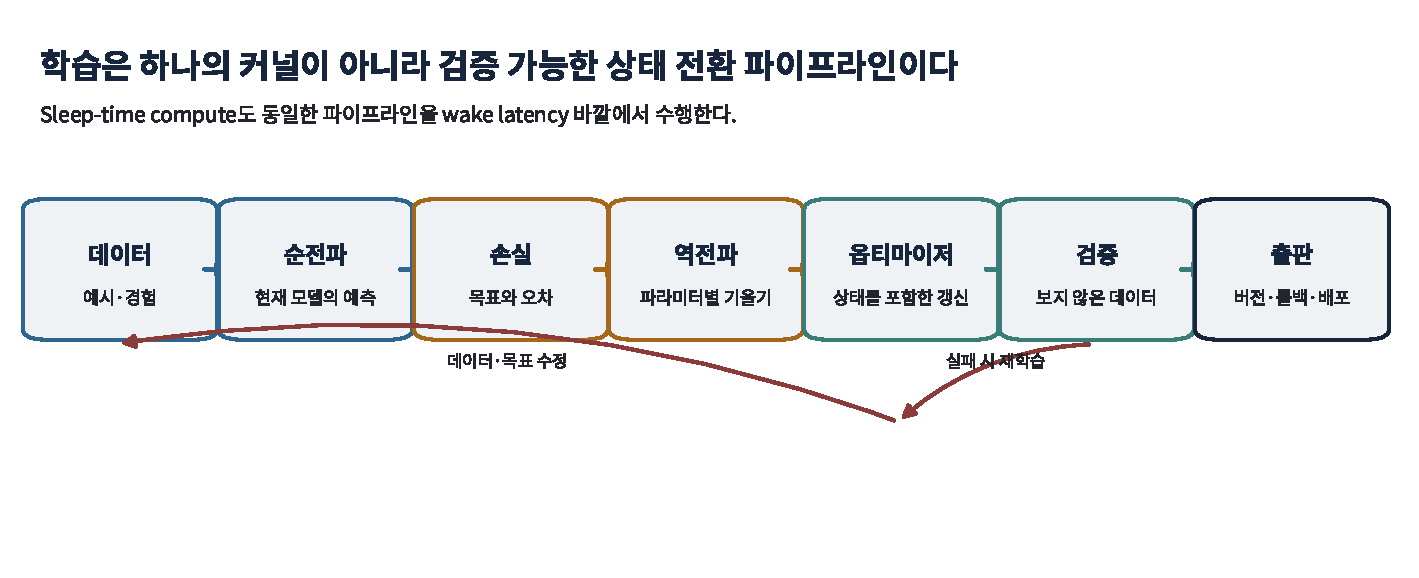
\includegraphics[width=\textwidth]{figures/learning-map.pdf}
  \caption{데이터에서 출판까지 이어지는 학습 상태 전환. Sleep-time compute는 이
  파이프라인의 일부를 응답 latency 경로 밖으로 옮기지만 검증 단계를 없애지 않는다.}
  \figsource{Original synthesis; context: SRC-STC-0030, SRC-STC-0014}{왼쪽의 데이터에서 오른쪽의 출판까지 일곱 상자가 화살표로 이어지고, 검증 실패 시 다시 데이터와 optimizer로 돌아간다.}
  \label{fig:bg-learning-map}
\end{figure}

\begin{keypoint}
학습 비용을 FLOPs만으로 세면 부족하다. 데이터 읽기, activation 보관, gradient와 optimizer
state, checkpoint 쓰기, validation inference, artifact 이동, rollback 보존까지가 한 번의
학습 상태 전환 비용이다.
\end{keypoint}
